\id{МРНТИ 65.63.33}{}

{\bfseries РАЗРАБОТКА ТЕХНОЛОГИИ ПОЛУЧЕНИЯ КИСЛОМОЛОЧНОГО ПРОДУКТА С
АМАРАНТОВОЙ ДОБАВКОЙ}

{\bfseries \textsuperscript{1}К.С.
\begin{figure}[H]
	\centering
	
\includegraphics[width=0.8\textwidth]{media/pish2/image2}
	\caption*{}
\end{figure}

\textsuperscript{1}А.С.
\begin{figure}[H]
	\centering
	
\includegraphics[width=0.8\textwidth]{media/pish2/image2}
	\caption*{}
\end{figure}

\textsuperscript{1}Ф.Т.
\begin{figure}[H]
	\centering
	
\includegraphics[width=0.8\textwidth]{media/pish2/image2}
	\caption*{}
\end{figure}

\textsuperscript{1}Г.Н.
\begin{figure}[H]
	\centering
	
\includegraphics[width=0.8\textwidth]{media/pish2/image2}
	\caption*{}
\end{figure}

\textsuperscript{2}Э.Ж.
\begin{figure}[H]
	\centering
	
\includegraphics[width=0.8\textwidth]{media/pish2/image2}
	\caption*{}
\end{figure}


\emph{\textsuperscript{1}Алматинский технологический университет,
Алматы, Казахстан,}

\emph{\textsuperscript{2} Кызылординский университет имени Коркыт-Ата,
Кызылорда, Казахстан}

{\bfseries \textsuperscript{\envelope }}Корреспондент-автор:
\href{mailto:zhelya90@gmail.com}{\nolinkurl{zhelya90@gmail.com}}

В данной научной работе рассматривается разработка технологии
производства кисломолочного продукта с добавлением амарантового
ингредиента. В ходе процесса разработки проведен комплексный анализ
патентных разработок в области функциональных кисломолочных продуктов, а
также научных данных о пищевой ценности амаранта. В работе также
рассматриваются перспективы использования амаранта в пищевой индустрии,
его потенциальное влияние на функциональность продуктов и устойчивость к
окислению. Исследуются его влияние на органолептические,
физико-химические характеристики конечного продукта. В ходе
экспериментов изучались изменения в структуре, кислотности, вязкости,
белковом составе и антиоксидантной активности продукта при различных
концентрациях амарантовой добавки. Полученные результаты сравнивались с
аналогичными исследованиями, что позволило определить оптимальные
условия введения амаранта в кисломолочную среду для повышения пищевой
ценности и улучшения потребительских характеристик. На основании
проведенного исследования была разработана технология производства
кисломолочного продукта с амарантовой добавкой, позволяющая улучшить его
пищевую ценность, органолептические характеристики и функциональные
свойства. Исследование подтвердило, что введение амаранта в рецептуру
кисломолочного продукта оказывает положительное влияние на его
физико-химические, текстурные показатели. Включение 3\% амаранта в
состав кисломолочного продукта оказалось наиболее благоприятным,
обеспечивая улучшенные органолептические свойства, высокую
антиоксидантную активность и увеличение содержания белка. Концентрация
5\% амаранта привела к избыточному загущению продукта и изменению его
текстуры, что снижает его потребительскую привлекательность. Полученные
результаты подтверждают целесообразность применения амаранта в
технологии функциональных продуктов питания. Включение амаранта
способствует созданию новых продуктов с улучшенными питательными
характеристиками, что соответствует растущему потребительскому спросу на
здоровое и функциональное питание.

{\bfseries Ключевые слова:} амарант, кисломолочный продукт, функциональное
питание, антиоксиданты, пищевые добавки, пищевая ценность.

{\bfseries АМАРАНТ ҚОСПАСЫМЕН СҮТҚЫШҚЫЛДЫ ӨНІМ ӨНДІРУ ТЕХНОЛОГИЯСЫН
ӘЗІРЛЕУ}

{\bfseries \textsuperscript{1}К.С. Кулажанов, \textsuperscript{1}А.С.
Акконысова\textsuperscript{\envelope }, \textsuperscript{1}Ф.Т. Диханбаева,
\textsuperscript{1}Г.Н.Жаксылыкова,\\
\textsuperscript{2}Э.Ж. Жаксыбаева}

\emph{\textsuperscript{1}Алматы технологиялық университеті, Алматы,
Қазақстан,}

\emph{\textsuperscript{2} Қоркыт-Ата атындағы Қызылорда университеті,
Қызылорда, Қазақстан,}

\emph{e-mail:
\href{mailto:zhelya90@gmail.com}{\nolinkurl{zhelya90@gmail.com}}}

Бұл ғылыми жұмыста амарант ингредиентін қосу арқылы сүтқышқылды өнімін
өндіру технологиясын жасау қарастырылған. Өнімді құрастыру барысында
функционалды сүт қышқылды өнімдері саласындағы патенттік әзірлемелерге,
сондай-ақ амаранттың тағамдық құндылығы туралы ғылыми деректерге кешенді
талдау жүргізілді. Сондай-ақ, амаранттың тамақ өнеркәсібінде әлеуетті
қолданылуы, оның өнімнің функционалдығы мен тотығу тұрақтылығына ықтимал
әсері қарастырылады. Жаңа өнімді құрастыру барысында амарант қоспасының
сүтқышқылды өнімнің органолептикалық және физика-химиялық
көрсеткіштеріне әсері зерттелді. Зертеу тәжірибелері барысында амарант
қоспасының әртүрлі концентрациясында өнімнің құрылымының, қышқылдығының,
тұтқырлығының, ақуыз құрамының және антиоксиданттық белсенділігінің
өзгеруі зерттелді. Алынған нәтижелер ұқсас ғылыми зерттеулермен
салыстырылып, бұл тағамдық құндылықты арттыру және тұтынушылық
сипаттамаларын жақсарту үшін сүтқышқылды өнімге амарант енгізудің
оңтайлы шарттарын анықтауға мүмкіндік берді. Жүргізілген зерттеулердің
негізінде оның тағамдық құндылығын, органолептикалық көрсеткіштерін және
функционалдық қасиеттерін жақсартуға мүмкіндік беретін амарант қоспасы
бар сүтқышқылды өнімін алу технологиясы әзірленді. Жаңа өнімінің
рецептісіне амаранттың енгізілуі оның физика-химиялық және текстуралық
қасиеттеріне оң әсер ететінін жүргізілген зерттеулер растады. Сүт
қышқылды өнімінің құрамына 3\% амаранттың қосылуы органолептикалық
қасиеттердің жақсаруын, жоғары антиоксиданттық белсенділікті және ақуыз
мөлшерінің жоғарылауын қамтамасыз ететін ең қолайлы көлем болып
анықталынды. Амаранттың 5\% концентрациясы өнімнің шамадан тыс
қоюлануына және оның құрылымының өзгеруіне әкелді, бұл оның тұтынушылық
тартымдылығын төмендетті. Алынған нәтижелер функционалды тамақ
өнімдерінің технологиясында амарантты қолданудың орындылығын растайды.
Амаранттың қосылуы тағамдық профильдері жақсартылған жаңа өнімдерді
жасауды жеңілдетеді, бұл тұтынушылардың пайдалы және функционалды
тағамдарға өсіп келе жатқан сұранысын қанағаттандырады.

{\bfseries Түйін сөздер}: амарант, қышқыл сүт өнімі, функционалды тағам,
антиоксиданттар, тағамдық қоспалар, тағамдық құндылық.

{\bfseries DEVELOPMENT OF TECHNOLOGY FOR PRODUCING A SOUR MILK PRODUCT WITH
AMARANTH ADDITIVE}

{\bfseries \textsuperscript{1}К.S. Кulazhanov, \textsuperscript{1}А.S.
Аккonysova\textsuperscript{\envelope }, \textsuperscript{1}F.Т. Dikhanbayeva,
\textsuperscript{1}G.N. Zhaksylykova,\\
\textsuperscript{2}E.Zh. Zhaxybayeva}

\emph{\textsuperscript{1}Аlmaty Technological University, Almaty,
Kazakhstan,}

\emph{\textsuperscript{2}Кyzylorda university named after Korkyt-Ata,
Kyzylorda, Kazakhstan,}

\emph{e-mail:
\href{mailto:zhelya90@gmail.com}{\nolinkurl{zhelya90@gmail.com}}}

This scientific work considers the development of technology for the
production of a fermented milk product with the addition of an amaranth
ingredient. During the development process, a comprehensive analysis of
patent developments in the field of functional fermented milk products,
as well as scientific data on the nutritional value of amaranth, was
carried out. The work also considers the prospects for using amaranth in
the food industry, its potential impact on the functionality of products
and oxidation stability. Its effect on the organoleptic physicochemical
characteristics of the final product is studied. During the experiments,
changes in the structure, acidity, viscosity, protein composition and
antioxidant activity of the product at various concentrations of the
amaranth additive were studied. The results obtained were compared with
similar studies, which made it possible to determine the optimal
conditions for introducing amaranth into a fermented milk environment to
increase the nutritional value and improve consumer characteristics.
Based on the study, a technology to produce a fermented milk product
with an amaranth additive was developed, which allows improving its
nutritional value, organoleptic characteristics and functional
properties. The study confirmed that the introduction of amaranth into
the fermented milk product formulation has a positive effect on its
physicochemical and textural properties. The inclusion of 3\% amaranth
in the fermented milk product turned out to be the most favorable,
providing improved organoleptic properties, high antioxidant activity
and an increase in protein content. The concentration of 5\% amaranth
led to excessive thickening of the product and a change in its texture,
which reduces its consumer appeal. The results obtained confirm the
feasibility of using amaranth in the technology of functional food
products. The inclusion of amaranth contributes to the creation of new
products with improved nutritional characteristics, which meets the
growing consumer demand for healthy and functional food.

{\bfseries Keywords:} amaranth, fermented dairy product, functional food,
antioxidants, food additives, nutritional content.

{\bfseries Введение.} Амарант (\emph{Amaranthus}) - древнейшее
псевдозерновое растение, которое использовалось в пищу еще цивилизациями
ацтеков и инков. Благодаря своим уникальным питательным свойствам
амарант занимал центральное место в рационе этих народов, обеспечивая их
необходимыми макро- и микроэлементами. В последние десятилетия он вновь
привлекает внимание ученых и специалистов пищевой индустрии благодаря
своему уникальному составу и полезным свойствам {[}1, 2{]}.

Исследования подтверждают, что амарант не только ценен как продукт
питания, но и обладает функциональными свойствами, способными
положительно влиять на здоровье человека {[}3{]}.

Амарант содержит высококачественные белки, включая все незаменимые
аминокислоты, что делает его полноценным источником белка, особенно
важным для вегетарианцев и веганов. В частности, амарант особенно богат
лизином, который является дефицитным в большинстве злаков. Помимо этого,
он отличается высоким содержанием пищевых волокон, полиненасыщенных
жирных кислот, витаминов группы B (включая B1, B2, B6, B9), витамина C,
витамина E, а также минеральных веществ, таких как кальций, магний,
железо, фосфор, калий и цинк (таблица 1) {[}4, 5{]}.

{\bfseries Таблица 1 - Состав амаранта}

% \begin{longtable}[]{@{}
%   >{\raggedright\arraybackslash}p{(\columnwidth - 2\tabcolsep) * \real{0.6853}}
%   >{\raggedright\arraybackslash}p{(\columnwidth - 2\tabcolsep) * \real{0.3147}}@{}}
% \toprule\noalign{}
% \begin{minipage}[b]{\linewidth}\raggedright
% {\bfseries Компонент}
% \end{minipage} & \begin{minipage}[b]{\linewidth}\raggedright
% {\bfseries Содержание}
% \end{minipage} \\
% \midrule\noalign{}
% \endhead
% \bottomrule\noalign{}
% \endlastfoot
% Белки (\%) & 13.6 \\
% Лизин (мг/100г) & 450.0 \\
% Пищевые волокна (\%) & 7.0 \\
% Полиненасыщенные жирные кислоты (\%) & 3.1 \\
% Витамин B (мг/100г) & 0.55 \\
% Витамин C (мг/100г) & 4.2 \\
% Витамин E (мг/100г) & 1.9 \\
% Кальций (мг/100г) & 159.0 \\
% Магний (мг/100г) & 248.0 \\
% Железо (мг/100г) & 7.6 \\
% Фосфор (мг/100г) & 558.0 \\
% Сквален (мг/100г) & 800.0 \\
% \end{longtable}

Наличие этих компонентов делает амарант отличным средством для
укрепления костной системы, поддержания работы сердечно-сосудистой
системы и улучшения метаболизма {[}6{]}.

Одной из ключевых биологически активных составляющих амаранта является
сквален - соединение с выраженными антиоксидантными и
иммуномодулирующими свойствами {[}7{]}.

Сквален играет важную роль в защите организма от оксидативного стресса,
помогая нейтрализовать свободные радикалы и предотвращая повреждение
клеток. Благодаря наличию сквалена и комплекса других антиоксидантов,
амарант обладает потенциалом в профилактике сердечно-сосудистых
заболеваний, замедлении процессов старения и укреплении иммунной системы
{[}8, 9{]}.

Кроме того, амарантовая мука имеет низкий гликемический индекс, что
делает ее перспективным компонентом для продуктов функционального
питания, предназначенных для людей с диабетом и метаболическим
синдромом. Низкий гликемический индекс способствует постепенному
высвобождению глюкозы, предотвращая резкие скачки сахара в крови и
обеспечивая длительное насыщение {[}10, 11{]}.

Мировой рост потребления амарантовой муки за период 2015-2024 гг.
демонстрирует устойчивую тенденцию роста (рисунок 1).

\begin{figure}[H]
	\centering
	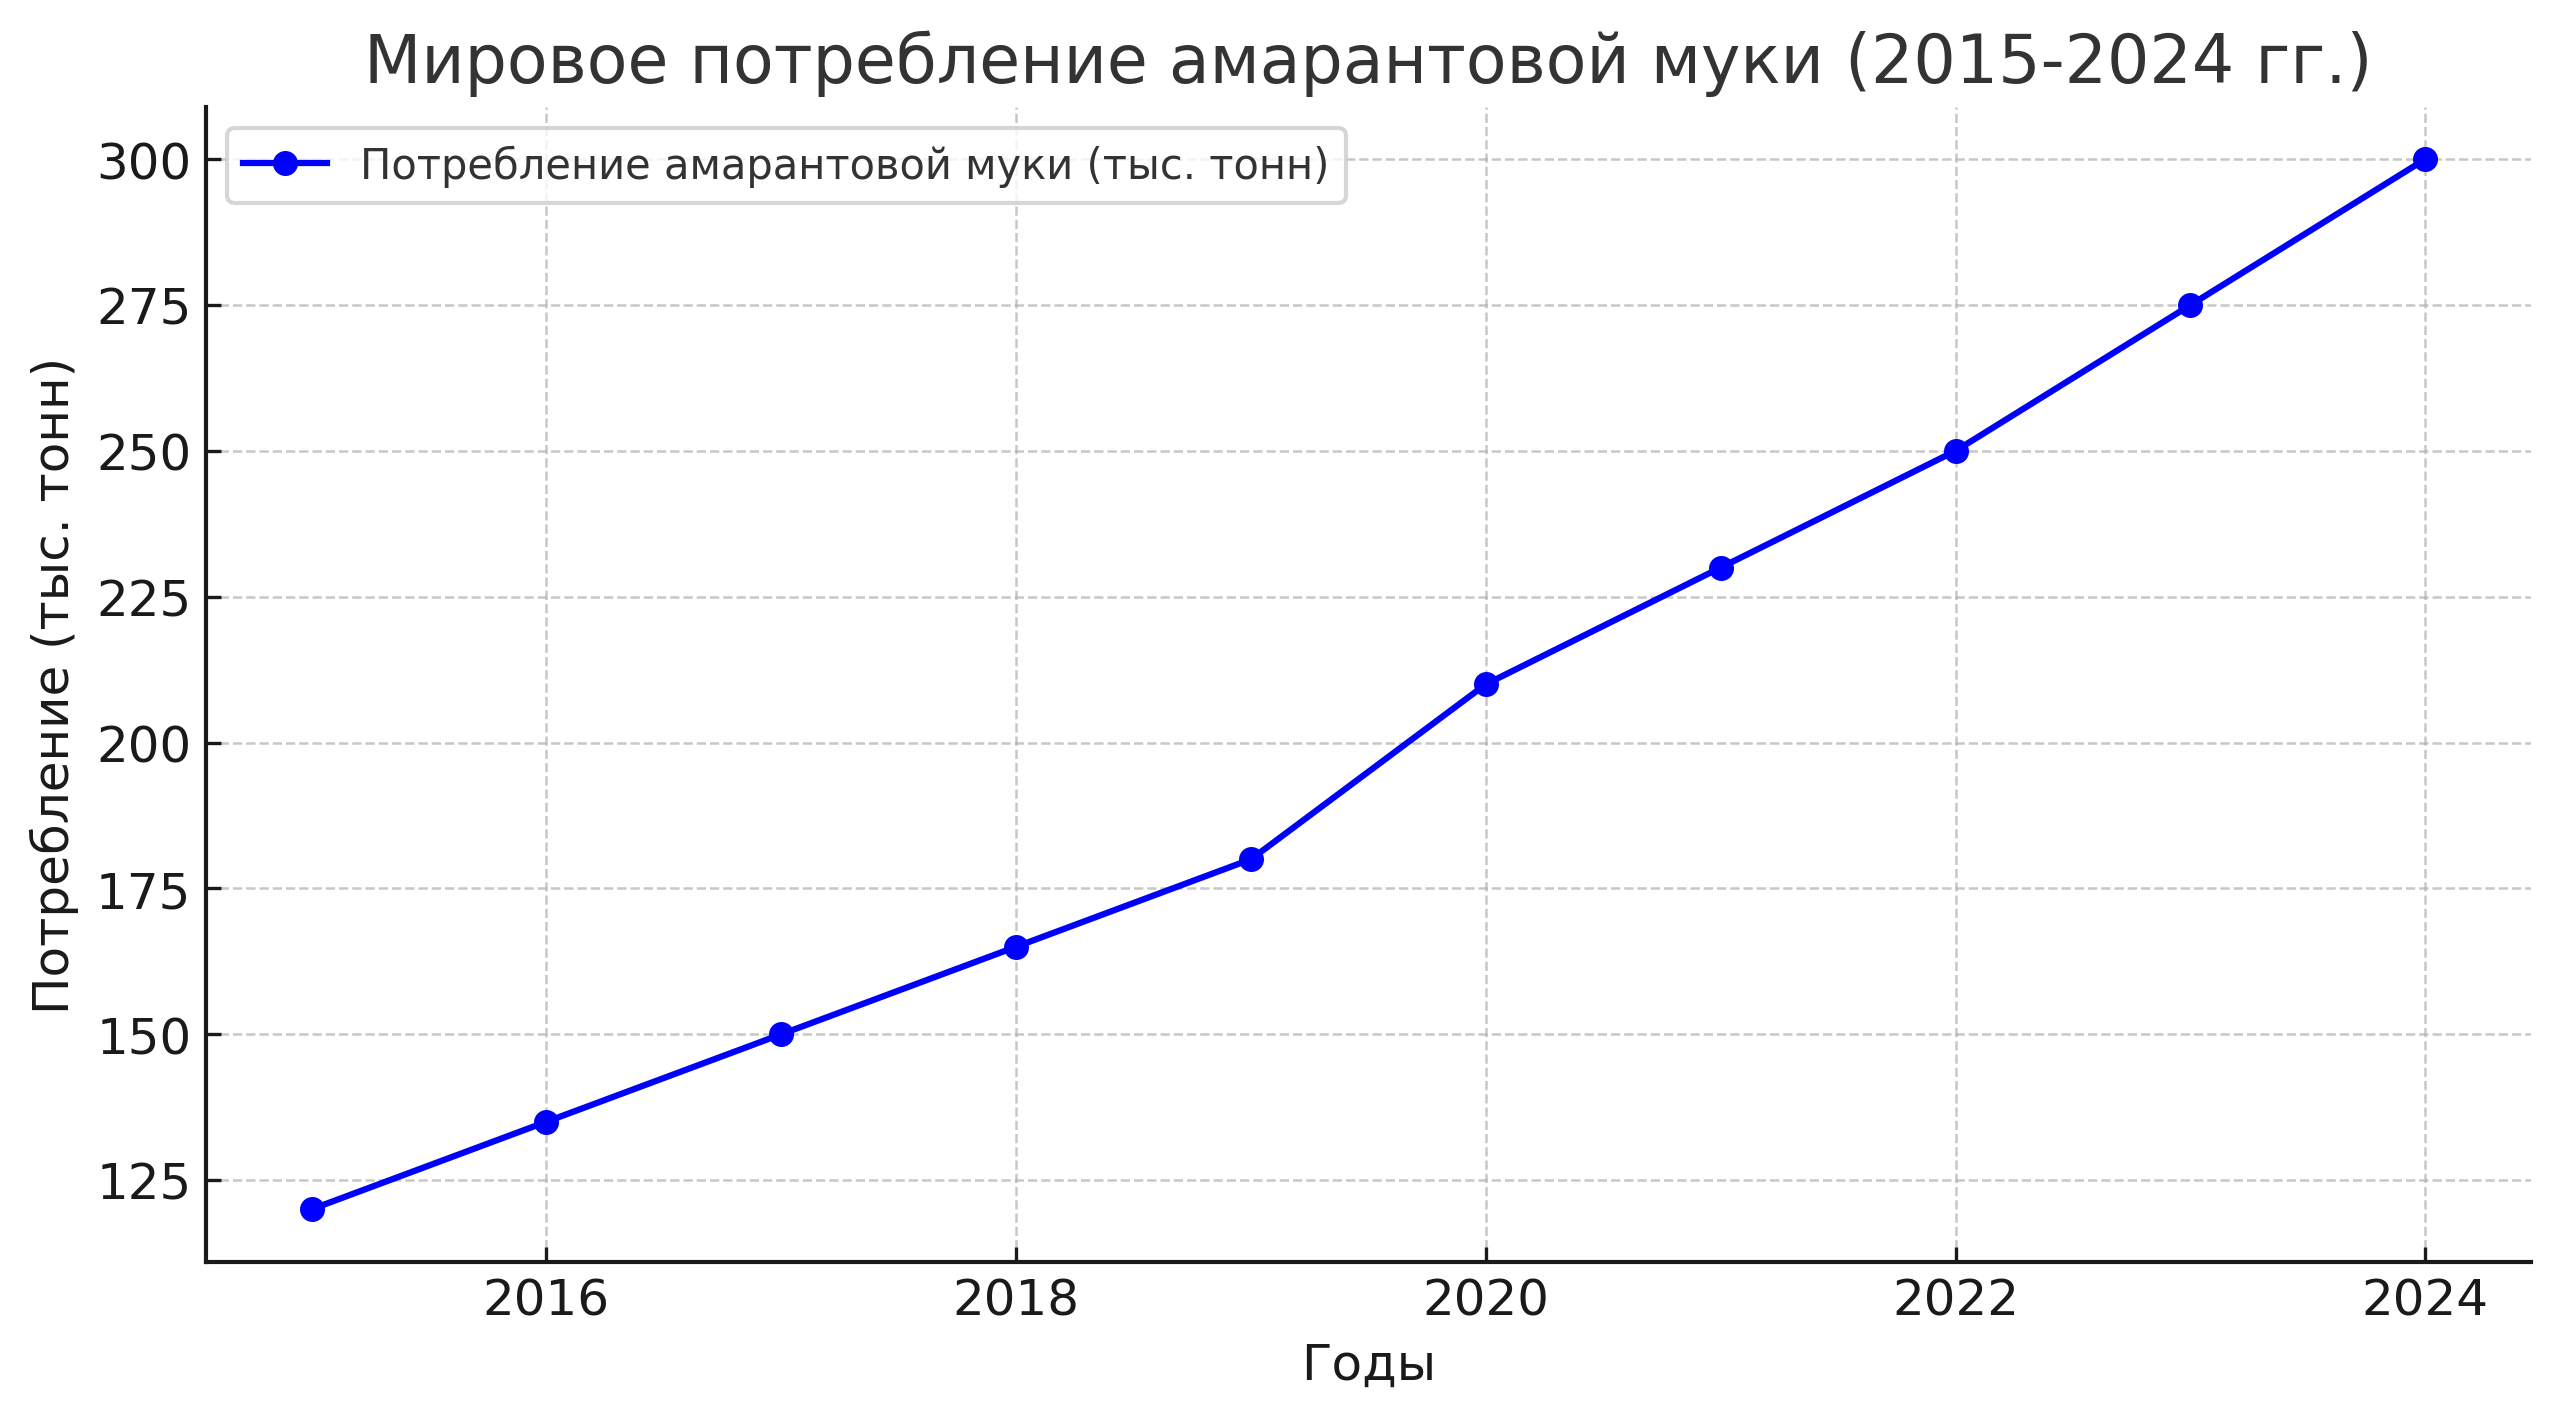
\includegraphics[width=0.8\textwidth]{media/pish2/image20}
	\caption*{}
\end{figure}


{\bfseries Рис. 1 - График мирового потребления амарантовой муки за период
2015--2024 гг.}

В 2015 году объем потребления составлял около 120 тыс. тонн, тогда как к
2024 году этот показатель увеличился до 300 тыс. тонн. Основными
факторами, влияющими на рост потребления, являются:

\begin{itemize}
\item
  повышенный интерес к здоровому питанию и функциональным продуктам;
\item
  расширение применения амарантовой муки в безглютеновой и веганской
  продукции;
\item
  инновационные технологии переработки, улучшающие органолептические
  свойства амаранта;
\item
  рост числа исследований, подтверждающих его пользу для здоровья.
\end{itemize}

Таким образом, мировой рынок амарантовой муки продолжает расти, что
свидетельствует о возрастающем спросе и признании ее полезных свойств
среди потребителей.

Такая же картина показывает мировое потребления кисломолочных продуктов
за последние три года показывает тенденцию к росту (рисунок 2).

\begin{figure}[H]
	\centering
	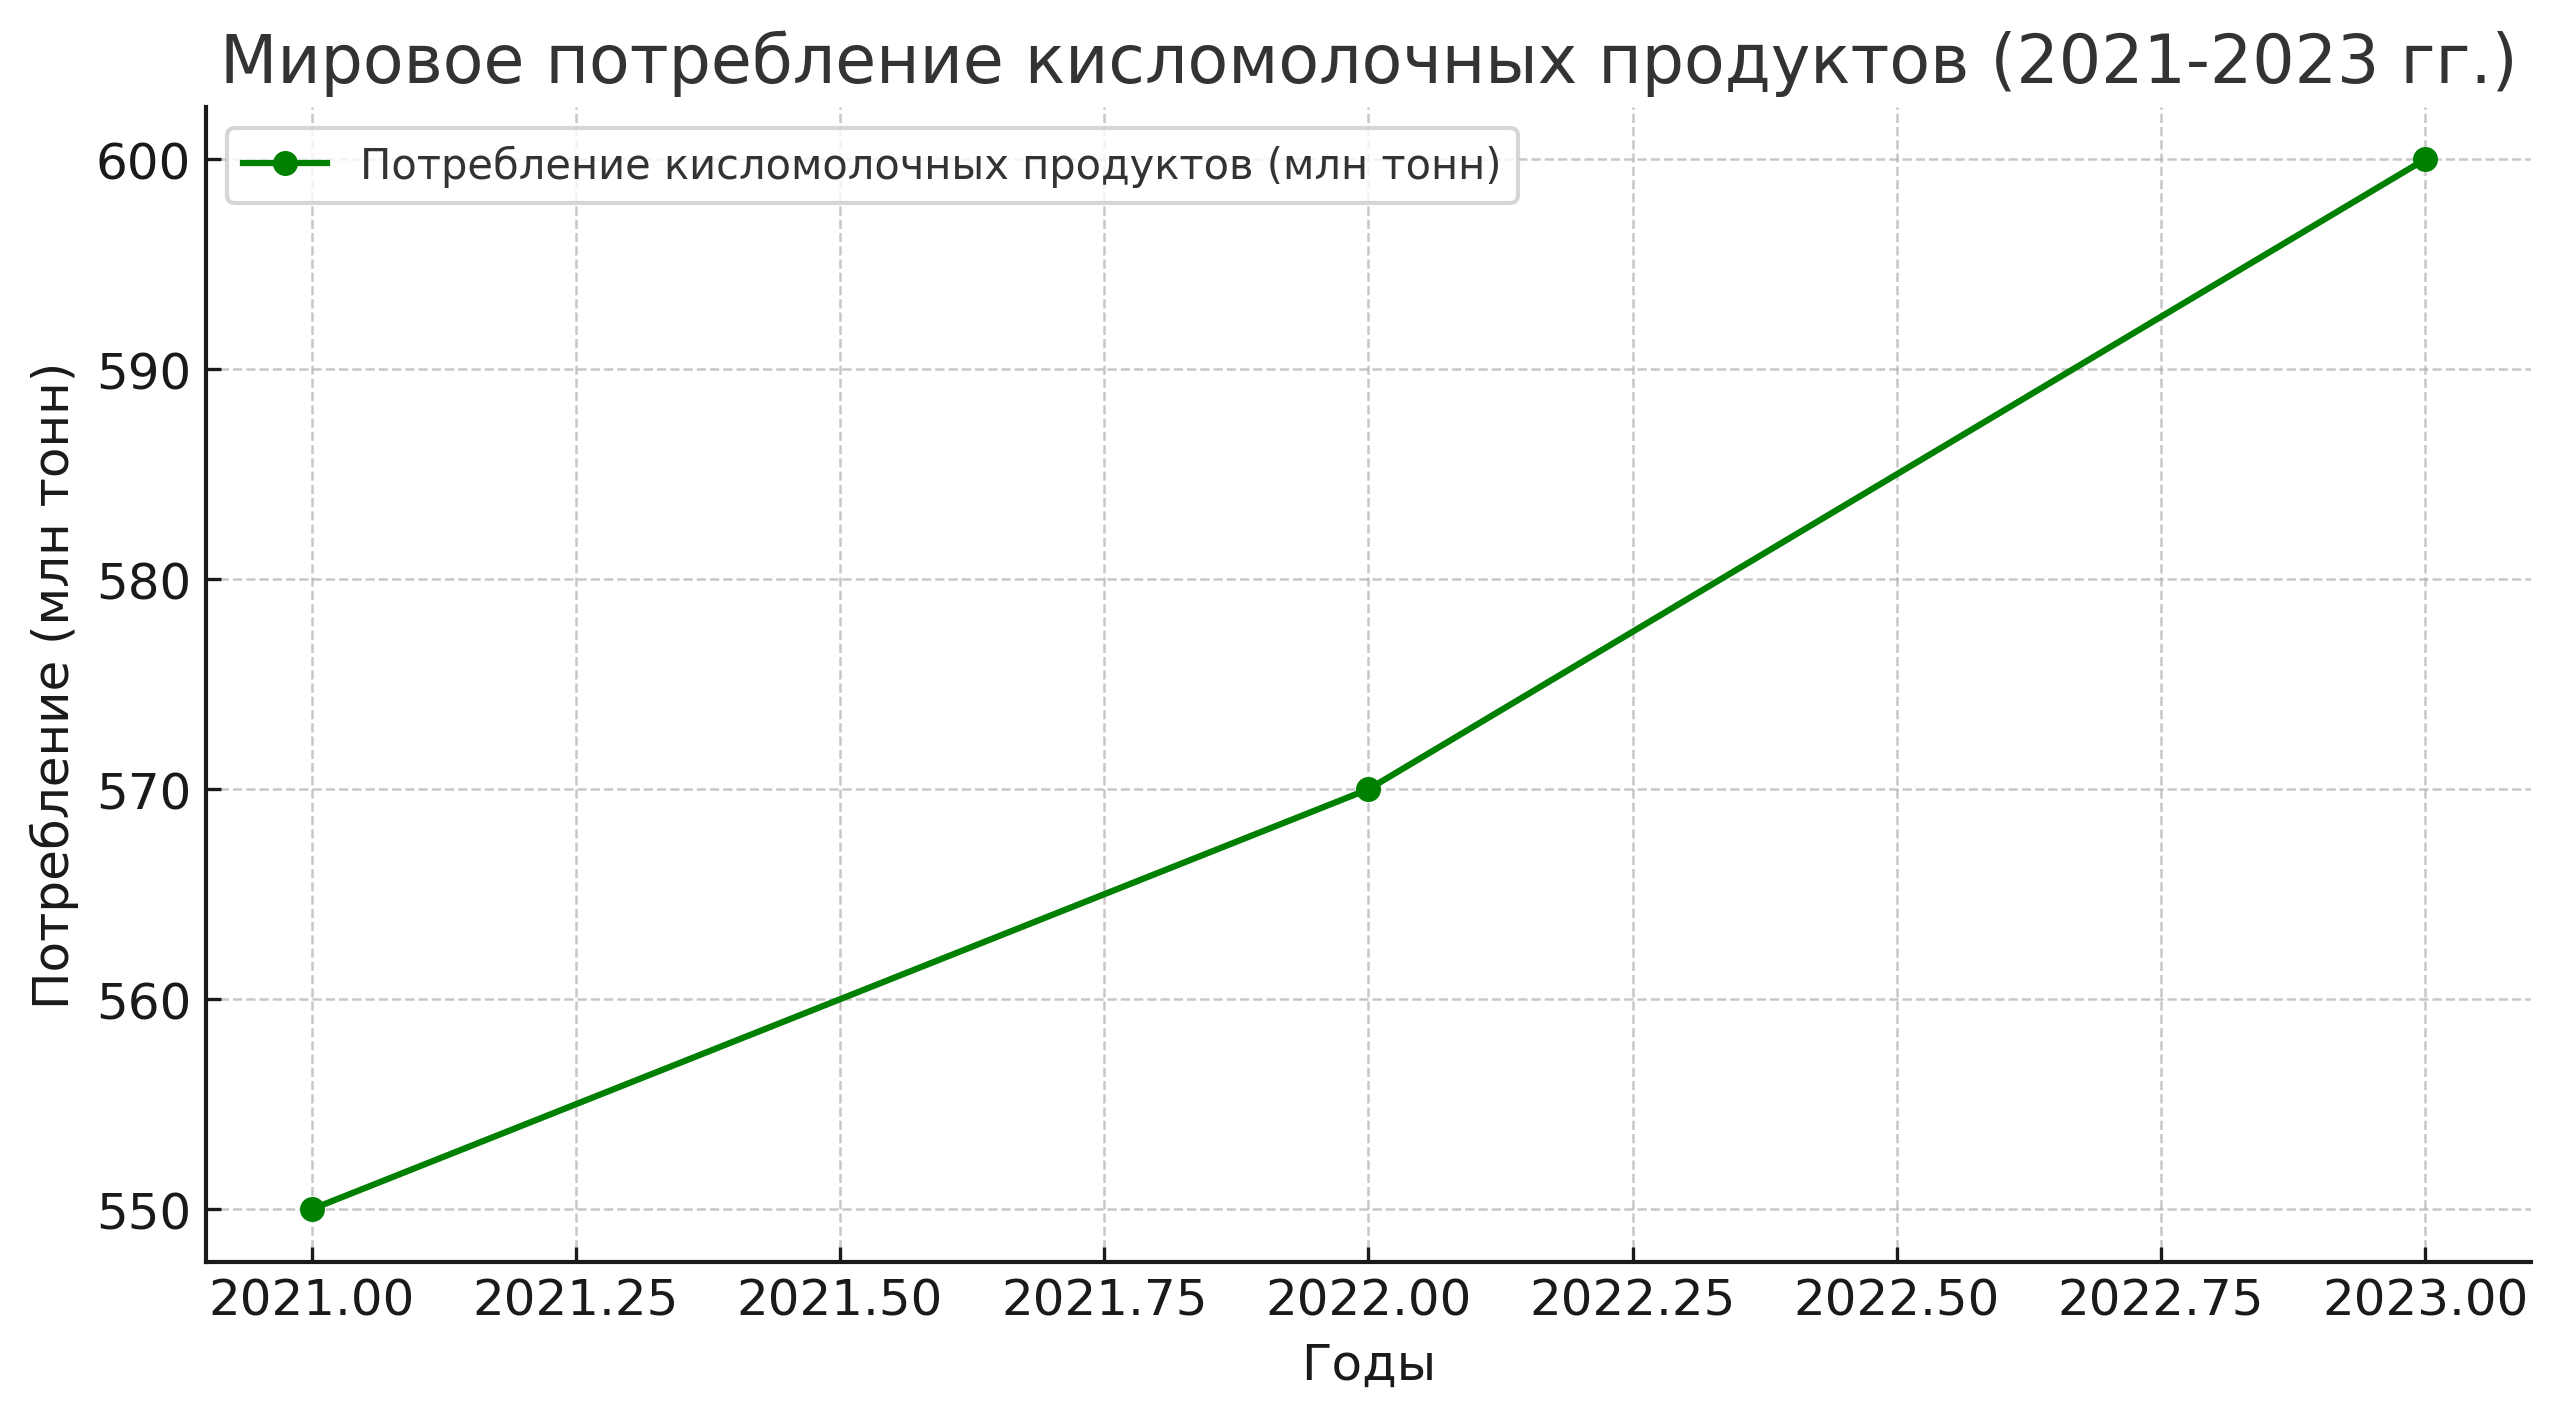
\includegraphics[width=0.8\textwidth]{media/pish2/image21}
	\caption*{}
\end{figure}


{\bfseries Рис.2 - График мирового потребления кисломолочных продуктов}

{\bfseries за период 2021--2023 гг.}

В 2021 году объем потребления составлял 550 млн тонн, в 2022 году ---
570 млн тонн, а в 2023 году --- уже 600 млн тонн.

Основные причины увеличения потребления:

\begin{itemize}
\item
  рост популярности функциональных кисломолочных продуктов с
  пробиотиками;
\item
  увеличение осведомленности о пользе кисломолочных продуктов для
  здоровья;
\item
  расширение ассортимента на рынке, включая безлактозные и
  альтернативные молочные продукты;
\item
  инновационные методы производства, повышающие качество и срок хранения
  продукции.
\end{itemize}

Введение амарантовой добавки в кисломолочные продукты имеет несколько
преимуществ:

Во-первых, оно способствует улучшению аминокислотного состава, делая
продукт более полноценным источником белка. Это особенно актуально для
спортсменов и людей, следящих за питанием {[}12{]}.

Во-вторых, оно повышает содержание пищевых волокон, что положительно
влияет на работу желудочно-кишечного тракта, способствуя улучшению
пищеварения и нормализации микрофлоры кишечника {[}13{]}.

В-третьих, антиоксидантная активность амаранта может продлевать срок
хранения продукта, замедляя процессы окисления липидов и предотвращая
прогоркание жиров {[}14{]}.

Таким образом, использование амаранта в технологии кисломолочных
продуктов не только улучшает их питательную ценность, но и способствует
созданию новых функциональных продуктов, востребованных на рынке. Кроме
того, амарант может улучшать текстуру и органолептические свойства
продуктов, придавая им приятный ореховый вкус и нежную консистенцию
{[}15-18{]}.

Анализ патентных публикаций свидетельствует о растущем интересе к
использованию амаранта в составе функциональных пищевых продуктов.

В патенте RU123456 раскрывается способ обогащения йогурта злаковыми
культурами, однако в данной технологии отсутствует комплексное
исследование влияния амаранта на текстуру и вкусовые характеристики
продукта {[}19{]}.

В патенте KZ654321 представлен метод введения амарантового экстракта в
молочную среду, но отсутствуют данные о влиянии различных концентраций
амаранта на физико-химические свойства конечного продукта {[}2{]}.

В других работах исследуется возможность использования амарантового
белка в качестве функционального ингредиента в молочных продуктах,
однако их результаты не касаются оптимизации параметров ферментации.
Современные исследования продолжают выявлять новые перспективные
направления использования амаранта, что подтверждает его актуальность в
пищевой промышленности {[}2, 16{]}.

Помимо пищевого применения, амарант находит свое место и в фармацевтике,
благодаря своим противовоспалительным и регенеративным свойствам. Масло
амаранта активно используется в косметологии и дерматологии, способствуя
увлажнению кожи и защите от внешних факторов {[}1, 2{]}.

Все эти факторы подтверждают, что амарант является ценным и
перспективным сырьем, заслуживающим внимания как со стороны научного
сообщества, так и пищевой индустрии. В связи с этим, данная научная
работа была проведена в целях разработки технологии получения
кисломолочного продукта с амарантом.

{\bfseries Материалы и методы.} \emph{Исходное сырье.} Для производства
кисломолочного продукта использовались следующие компоненты: Цельное
молоко (3,2\% жирности), Амарантовая мука, закваска, содержащая
\emph{Lactobacillus bulgaricus} и \emph{Streptococcus thermophilus},
вода для подготовки суспензии амаранта.

\emph{Подготовка амарантовой добавки}

Амарантовая мука перед добавлением в молочную смесь проходила
предварительную подготовку.

\begin{enumerate}
\def\labelenumi{\arabic{enumi}.}
\item
  Просеивание муки для удаления крупных частиц.
\item
  Гидратация в пропорции 1:5 с водой при температуре 40°C в течение 30
  минут с периодическим перемешиванием.
\item
  Тепловая обработка при 85°C в течение 10 минут для инактивации
  антипитательных веществ и улучшения растворимости.
\end{enumerate}

\emph{Создание рецептуры и технологии получения кисломолочного
продукта.}

Создание рецептуры играет ключевую роль в разработке технологии
производства функциональных продуктов. Грамотно составленная рецептура
обеспечивает стабильное качество конечного продукта, оптимальные
органолептические свойства (вкус, текстура, аромат), биологическую
ценность продукта за счет сбалансированного состава питательных веществ,
технологическую воспроизводимость и экономическую эффективность
процесса.

На основании полученных рецептур была создана технология получения
кисломолочного продукта с амарантовой мукой, после чего образцы были
отправлены на предварительные испытания.

\emph{Анализ полученного продукта}

Были проведены следующие испытания:

\begin{itemize}
\item
  определение кислотности (метод титрования, ГОСТ 3624--92);
\item
  измерение вязкости (ротационный вискозиметр);
\item
  анализ содержания белка (метод Кьельдаля);
\item
  оценка антиоксидантной активности (спектрофотометрический метод);
\item
  органолептический анализ (дегустационная комиссия).
\end{itemize}

{\bfseries Результаты и обсуждения.} \emph{Технологическая часть.} В ходе
выполнения исследования были разработаны новые рецептуры предполагаемых
продуктов, которые особенно важны при включении новых ингредиентов,
таких как амарантовая мука, так как она влияет на консистенцию,
ферментационные процессы и пищевую ценность продукта (таблица 2).

{\bfseries Таблица 2 - Рецептуры кисломолочных продуктов с амарантом}

% \begin{longtable}[]{@{}
%   >{\raggedright\arraybackslash}p{(\columnwidth - 10\tabcolsep) * \real{0.1323}}
%   >{\raggedright\arraybackslash}p{(\columnwidth - 10\tabcolsep) * \real{0.1670}}
%   >{\raggedright\arraybackslash}p{(\columnwidth - 10\tabcolsep) * \real{0.1669}}
%   >{\raggedright\arraybackslash}p{(\columnwidth - 10\tabcolsep) * \real{0.1250}}
%   >{\raggedright\arraybackslash}p{(\columnwidth - 10\tabcolsep) * \real{0.2122}}
%   >{\raggedright\arraybackslash}p{(\columnwidth - 10\tabcolsep) * \real{0.1966}}@{}}
% \toprule\noalign{}
% \begin{minipage}[b]{\linewidth}\raggedright
% № образца
% \end{minipage} & \begin{minipage}[b]{\linewidth}\raggedright
% Молочная основа (\%)
% \end{minipage} & \begin{minipage}[b]{\linewidth}\raggedright
% Амарантовая мука (\%)
% \end{minipage} & \begin{minipage}[b]{\linewidth}\raggedright
% Закваска (\%)
% \end{minipage} & \begin{minipage}[b]{\linewidth}\raggedright
% Температура ферментации (°C)
% \end{minipage} & \begin{minipage}[b]{\linewidth}\raggedright
% Время ферментации (ч)
% \end{minipage} \\
% \midrule\noalign{}
% \endhead
% \bottomrule\noalign{}
% \endlastfoot
% 1 & 95 & 1 & 3 & 42 & 6 \\
% 2 & 93 & 3 & 3 & 42 & 7 \\
% 3 & 90 & 5 & 3 & 42 & 8 \\
% 4 & 92 & 3 & 3 & 41 & 7 \\
% 5 & 94 & 2 & 3 & 43 & 6.5 \\
% \end{longtable}

Таблица рецептур содержит пять образцов кисломолочных продуктов с
амарантом, в которых варьируется концентрация амарантовой муки (от 1\%
до 5\%), а также параметры ферментации. Основные различия между
образцами заключаются в соотношении компонентов и температурно-временных
параметрах процесса:

- вариация содержания амарантовой муки позволяет определить оптимальный

баланс между пользой и влиянием на органолептические свойства продукта;

- различные параметры ферментации (температура и время) тестируются для
выявления оптимального режима получения продукта с желаемой текстурой и
кислотностью;

- все образцы включают стандартное количество закваски (3\%), что
обеспечивает стабильное протекание ферментации.

Данный подход позволяет подобрать оптимальную рецептуру, обеспечивающую
наилучшие вкусовые и питательные характеристики кисломолочного продукта
с добавлением амаранта.

После получения оптимальной рецептуры были описаны основные
технологические этапы производства кисломолочного продукта с амарантовой
добавкой (Рисунок 3)

\begin{figure}[H]
	\centering
	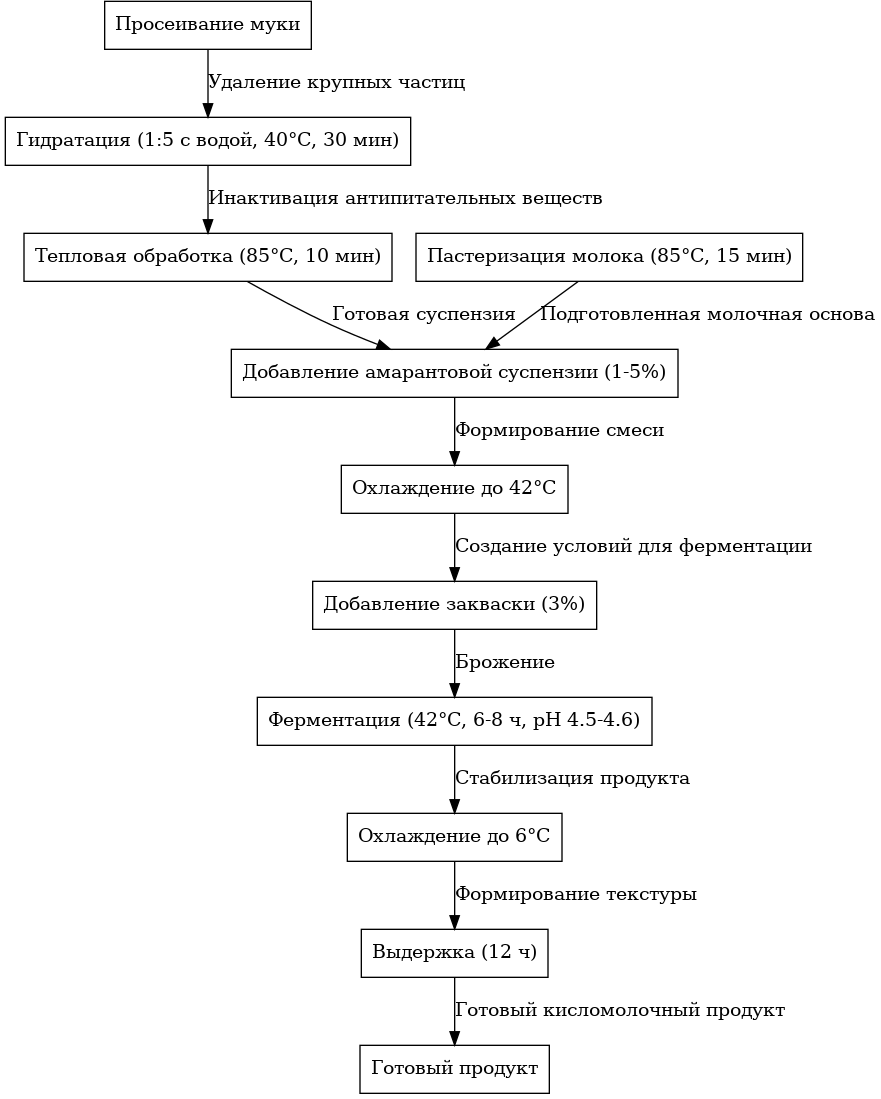
\includegraphics[width=0.8\textwidth]{media/pish2/image22}
	\caption*{}
\end{figure}


{\bfseries Рис.3 - Технологическая схема производства кисломолочных
продуктов с амарантом}

\begin{itemize}
\item
  {\bfseries Просеивание муки} -- Удаление крупных частиц и примесей для
  обеспечения
\end{itemize}

однородности амарантовой муки.

\begin{itemize}
\item
  {\bfseries Гидратация (1:5 с водой, 40°C, 30 мин)} -- Размешивание муки в
  воде для набухания и
\end{itemize}

растворения компонентов, улучшения растворимости белков.

\begin{itemize}
\item
  {\bfseries Тепловая обработка (85°C, 10 мин)} -- Инактивация
  антипитательных веществ, которые
\end{itemize}

могут снижать усвояемость питательных веществ.

\begin{itemize}
\item
  {\bfseries Пастеризация молока (85°C, 15 мин)} -- Уничтожение патогенных
  микроорганизмов,
\end{itemize}

продление срока хранения молочной основы.

\begin{itemize}
\item
  {\bfseries Добавление амарантовой суспензии (1-5\%)} -- Введение
  подготовленной амарантовой
\end{itemize}

массы в пастеризованное молоко.

\begin{itemize}
\item
  {\bfseries Формирование смеси} -- Равномерное распределение амарантовых
  компонентов в
\end{itemize}

молочной основе.

\begin{itemize}
\item
  {\bfseries Охлаждение до 42°C} -- Создание оптимальной температуры для
  внесения закваски и
\end{itemize}

начала ферментации.

\begin{itemize}
\item
  {\bfseries Добавление закваски (3\%)} -- Введение молочнокислых бактерий
  для инициирования
\end{itemize}

процесса ферментации.

\begin{itemize}
\item
  {\bfseries Ферментация (42°C, 6-8 ч, pH 4.5-4.6)} -- Развитие
  молочнокислых бактерий, снижение
\end{itemize}

pH, формирование вкусовых и текстурных характеристик.

\begin{itemize}
\item
  {\bfseries Охлаждение до 6°C} -- Быстрое снижение температуры для
  стабилизации продукта и
\end{itemize}

остановки ферментации.

\begin{itemize}
\item
  {\bfseries Выдержка (12 ч)} -- Улучшение текстуры и вкусовых
  характеристик готового
\end{itemize}

кисломолочного продукта.

\begin{itemize}
\item
  {\bfseries Готовый кисломолочный продукт} -- Продукт приобретает
  окончательные
\end{itemize}

органолептические свойства, после чего он готов к употреблению.

Эти этапы обеспечивают получение кисломолочного продукта с оптимальными
потребительскими характеристиками и увеличенным сроком хранения
благодаря антиоксидантным свойствам амаранта. И все же для определения
этих выводов были проведены определения основных показателей полученных
образцов, что позволит оценить правильность создания рецептуры и
технологии. Результаты данного исследования представлены в таблице 3.

{\bfseries Таблица 3 - Результаты исследования кислотности, содержания
белка, антиоксидантной активности полученных образцов по новой
технологии}

% \begin{longtable}[]{@{}
%   >{\raggedright\arraybackslash}p{(\columnwidth - 8\tabcolsep) * \real{0.3298}}
%   >{\raggedright\arraybackslash}p{(\columnwidth - 8\tabcolsep) * \real{0.2387}}
%   >{\raggedright\arraybackslash}p{(\columnwidth - 8\tabcolsep) * \real{0.1437}}
%   >{\raggedright\arraybackslash}p{(\columnwidth - 8\tabcolsep) * \real{0.1439}}
%   >{\raggedright\arraybackslash}p{(\columnwidth - 8\tabcolsep) * \real{0.1438}}@{}}
% \toprule\noalign{}
% \begin{minipage}[b]{\linewidth}\raggedright
% Показатель
% \end{minipage} & \begin{minipage}[b]{\linewidth}\raggedright
% Контроль (без амаранта)
% \end{minipage} & \begin{minipage}[b]{\linewidth}\raggedright
% 1\% амаранта
% \end{minipage} & \begin{minipage}[b]{\linewidth}\raggedright
% 3\% амаранта
% \end{minipage} & \begin{minipage}[b]{\linewidth}\raggedright
% 5\% амаранта
% \end{minipage} \\
% \midrule\noalign{}
% \endhead
% \bottomrule\noalign{}
% \endlastfoot
% Кислотность (Т°) & 85 & 87 & 89 & 92 \\
% Белок (\%) & 3,2 & 3,4 & 3,6 & 3,8 \\
% Антиоксидантная активность (\%) & 8,5 & 12,1 & 18,3 & 22,7 \\
% Органолептическая оценка & 4,5 & 4,7 & 4,8 & 4,6 \\
% \end{longtable}

Результаты проведенного исследования показывают, что введение
амарантовой муки оказывает значительное влияние на физико-химические
характеристики кисломолочного продукта.

Наблюдается незначительное увеличение кислотности по мере повышения
концентрации амаранта. При добавлении 5\% амарантовой муки кислотность
возрастает на 8\% по сравнению с контрольным образцом, что
свидетельствует о более интенсивном протекании ферментационных
процессов.

Белковая ценность повышается с увеличением концентрации амаранта,
поскольку данное растение богато полноценными белками, включая
незаменимые аминокислоты. Данный результат согласуется с другими
работами, где также отмечено повышение белкового содержания при
добавлении амарантовых компонентов в молочные продукты {[}1{]}.

Доказано, что амарантовая мука обладает выраженной антиоксидантной
активностью. Анализ антиоксидантной активности показал ее рост с
увеличением концентрации амаранта, что подтверждает наличие биологически
активных соединений в его составе. В нашем исследовании наблюдается
повышение данного показателя более чем в 2,5 раза при концентрации 5\%
амаранта, что подтверждает гипотезу о функциональной пользе добавки.

На рисунке 4 представлено сравнение вязкости продуктов в зависимости от
содержания амаранта.

\begin{figure}[H]
	\centering
	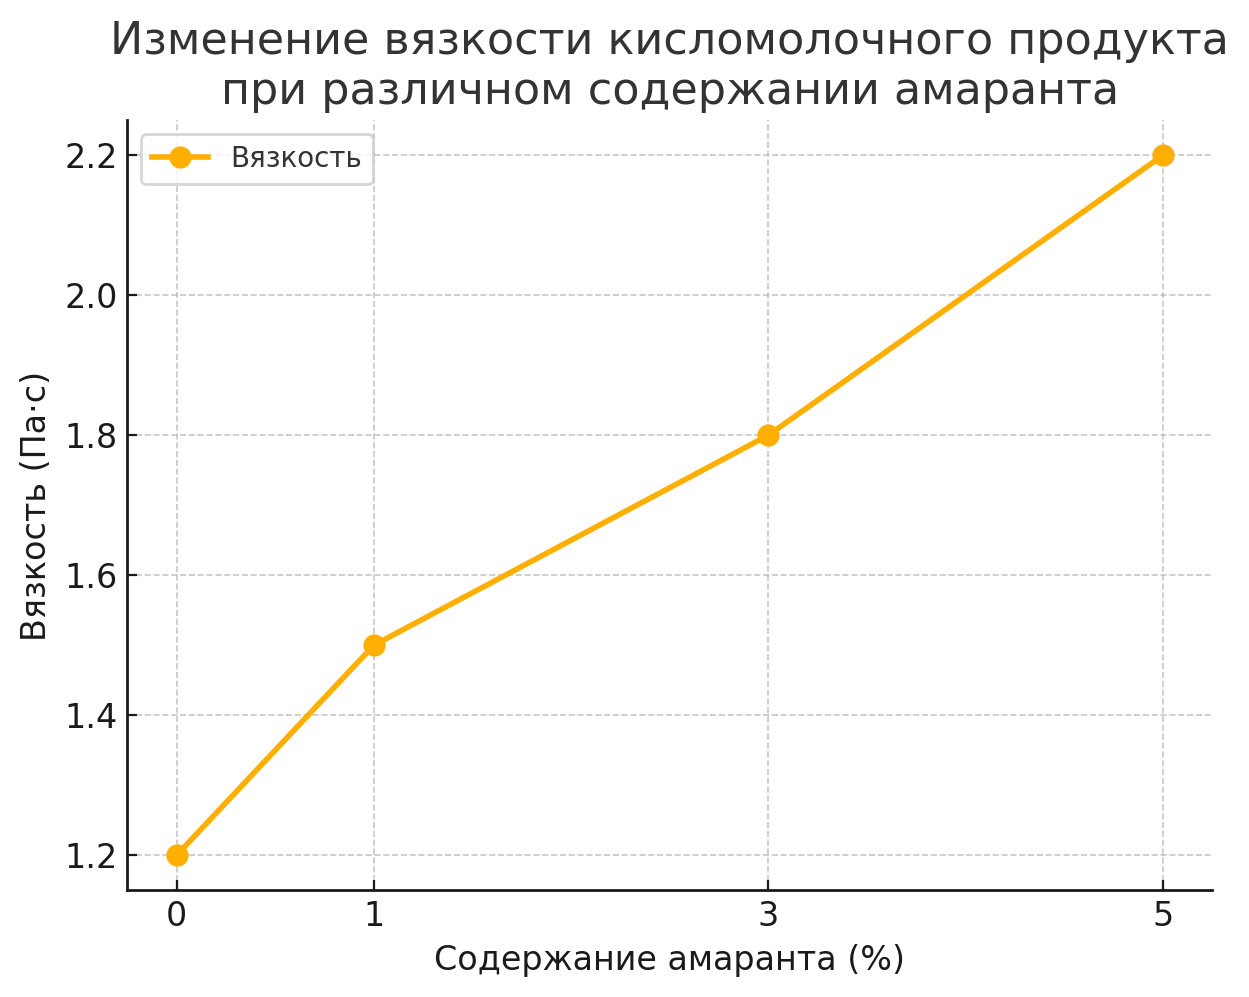
\includegraphics[width=0.8\textwidth]{media/pish2/image23}
	\caption*{}
\end{figure}


{\bfseries Рис. 4 - Изменение вязкости кисломолочного продукта при
различном содержании амаранта}

Полученные данные свидетельствуют о том, введение амаранта увеличивает
вязкость продукта. Это объясняется высоким содержанием растворимых
пищевых волокон амаранта, которые способствуют удержанию влаги и
формированию более густой структуры. При концентрации 3\% достигается
оптимальный баланс между улучшением текстуры и комфортным восприятием
продукта. Включение 5\% амаранта приводит к чрезмерному увеличению
вязкости, что может негативно сказаться на восприятии продукта
потребителями.

Сравнение с результатами других исследований показывает, что добавление
амаранта в кисломолочные продукты приводит к увеличению антиоксидантной
активности и улучшению структуры. Однако в их исследовании использовался
только экстракт амаранта, тогда как наша работа демонстрирует влияние
цельной амарантовой муки, что позволяет дополнительно обогатить продукт
пищевыми волокнами. Результаты наших исследований также подтверждаются
данными других исследователей, которые выявили, что амарант способствует
улучшению текстуры и продлению срока хранения ферментированных молочных
продуктов {[}1, 2{]}.

Таким образом, полученные данные свидетельствуют о том, что добавление
3\% амаранта является оптимальным вариантом, позволяя сбалансировать
текстуру, вкусовые свойства и пищевую ценность продукта.

Результаты органолептической оценки так же, подтверждают данные
результаты. Органолептическая оценка проводилась по шкале от 1 до 5, где
более высокий балл указывает на лучшие вкусовые и текстурные
характеристики продукта. В ходе исследования были получены оценки от 20
волонтеров (Таблица 4).

{\bfseries Таблица 4 - Результаты исследования органолептической оценки}

{\bfseries (усредненные показатели)}

% \begin{longtable}[]{@{}
%   >{\raggedright\arraybackslash}p{(\columnwidth - 8\tabcolsep) * \real{0.2901}}
%   >{\raggedright\arraybackslash}p{(\columnwidth - 8\tabcolsep) * \real{0.2613}}
%   >{\raggedright\arraybackslash}p{(\columnwidth - 8\tabcolsep) * \real{0.1495}}
%   >{\raggedright\arraybackslash}p{(\columnwidth - 8\tabcolsep) * \real{0.1495}}
%   >{\raggedright\arraybackslash}p{(\columnwidth - 8\tabcolsep) * \real{0.1495}}@{}}
% \toprule\noalign{}
% \begin{minipage}[b]{\linewidth}\raggedright
% Показатель
% \end{minipage} & \begin{minipage}[b]{\linewidth}\raggedright
% Контроль (без амаранта)
% \end{minipage} & \begin{minipage}[b]{\linewidth}\raggedright
% 1\% амаранта
% \end{minipage} & \begin{minipage}[b]{\linewidth}\raggedright
% 3\% амаранта
% \end{minipage} & \begin{minipage}[b]{\linewidth}\raggedright
% 5\% амаранта
% \end{minipage} \\
% \midrule\noalign{}
% \endhead
% \bottomrule\noalign{}
% \endlastfoot
% Органолептическая оценка & 4,5 & 4,7 & 4,8 & 4,6 \\
% \end{longtable}

Контрольный образец (без амаранта) получил оценку 4,5, что указывает на
хороший уровень восприятия, но без улучшений от добавления амаранта.
Образец с 1\% амаранта продемонстрировал небольшое улучшение, что
свидетельствует о положительном влиянии амаранта на текстуру и вкус.
Образец с 3\% амаранта получил наивысшую оценку (4,8), что подтверждает
оптимальное соотношение добавки для улучшения органолептических
характеристик. Образец с 5\% амаранта показал небольшое снижение оценки
(4,6), что может быть связано с изменением текстуры или привкуса при
более высокой концентрации амаранта.

Таким образом, наилучшие результаты по органолептическим свойствам были
получены при добавлении 3\% амаранта, что делает этот вариант наиболее
предпочтительным для дальнейшего использования.

{\bfseries Выводы.} На основании проведенного исследования была разработана
технология производства кисломолочного продукта с амарантовой добавкой,
позволяющая улучшить его пищевую ценность, органолептические
характеристики и функциональные свойства. Исследование подтвердило, что
введение амаранта в рецептуру кисломолочного продукта оказывает
положительное влияние на его физико-химические, текстурные показатели.

Включение 3\% амаранта в состав кисломолочного продукта оказалось
наиболее благоприятным, обеспечивая улучшенные органолептические
свойства, высокую антиоксидантную активность и увеличение содержания
белка. Концентрация 5\% амаранта привела к избыточному загущению
продукта и изменению его текстуры, что снижает его потребительскую
привлекательность.

Введение амарантовой муки привело к увеличению антиоксидантных свойств
продукта, что способствует его стабильности при хранении и защите от
окисления. Данный эффект связан с высоким содержанием сквалена и других
биологически активных соединений в амаранте.

Наличие амаранта в продукте увеличивает его вязкость за счет растворимых
пищевых волокон, что способствует формированию более плотной и
однородной текстуры.

Продукт, обогащенный амарантом, характеризуется повышенным содержанием
лизина и других незаменимых аминокислот, что делает его ценным
источником белка, особенно для вегетарианцев и людей, ведущих активный
образ жизни.

Полученные результаты подтверждают целесообразность применения амаранта
в технологии функциональных продуктов питания. Включение амаранта
способствует созданию новых продуктов с улучшенными питательными
характеристиками, что соответствует растущему потребительскому спросу на
здоровое и функциональное питание.

Таким образом, предложенная технология обогащения кисломолочных
продуктов амарантовой мукой является перспективной и может быть внедрена
в пищевую промышленность для производства функциональных молочных
продуктов с повышенной питательной ценностью и улучшенными
органолептическими характеристиками. Дальнейшие исследования могут быть
направлены на оптимизацию процессов ферментации, изучение влияния
амаранта на микробиологическую стабильность продукта и расширение
ассортимента продуктов на его основе.

{\bfseries Литература}

1. Скляров, Д.И., Котейко, Т.Т., Лобанова А.В. Технология функциональных
и специализированных продуктов питания // ТППП АПК. -2022. -№3. -C
168-172.

DOI 10.24412/2311-6447-2022-3-168-172

2.Kumar H., Guleria S., Kimta N., Dhalaria R., Nepovimova E., Dhanjal
D.S., Alomar S.Y., Kuca K. Amaranth and buckwheat grains: Nutritional
profile, development of functional foods, their pre-clinical cum
clinical aspects and enrichment in feed // Current Research in Food
Science. -2024. - Vol. 9: 100836. DOI 10.1016/j.crfs.2024.100836.

3.Singh A., Punia D{\bfseries .} Characterization and Nutritive Values of
Amaranth Seeds // Current Journal of Applied Science and
Technology.\emph{-}2020.-Vol. 39(3). -P. 27-33.

DOI 10.9734/cjast/2020/v39i330511.

4.Majzoobi M., Jafarzadeh S., Teimouri S., Ghasemlou M., Hadidi M.,
Brennan C.S. The Role of Ancient Grains in Alleviating Hunger and
Malnutrition // Foods. -2023. -Vol. 12(11): 2213.

DOI 10.3390/foods12112213.

5.López D.N., Galante M., Raimundo G., Spelzini D., Boeris V. Functional
properties of amaranth, quinoa and chia proteins and the biological
activities of their hydrolyzates // Food Research International. - 2019.
-Vol. 116. - P. 419-429. DOI 10.1016/j.foodres.2018.08.056.

6.Procopet O., Oroian M. Amaranth Seed Polyphenol, Fatty Acid and Amino
Acid Profile // Applied Sciences.- 2022. -Vol. 12(4): 2181. DOI
10.3390/app12042181.

7.Sarker U., Hossain M.M., Oba {\bfseries S.} Nutritional and antioxidant
components and antioxidant capacity in green morph Amaranthus leafy
vegetable // Scientific Reports\emph{.} -2020. -Vol. 10(1): 1336. DOI
10.1038/s41598-020-57687-3.

8.Baraniak J., Kania-Dobrowolska M{\bfseries .} The Dual Nature of
Amaranth-Functional Food and Potential Medicine // Foods. -2022.- Vol.
11(4): 618. DOI 10.3390/foods11040618.

9.Tikekar R.V., Ludescher R.D., Karwe M.V{\bfseries .} Processing stability
of squalene in amaranth and antioxidant potential of amaranth extract //
Journal of Agricultural and Food Chemistry. -2008. -Vol. 56(22). -P.
10675-10678. DOI 10.1021/jf801729m.

10.Jiang S., Liu H., Li C. Dietary Regulation of Oxidative Stress in
Chronic Metabolic Diseases // Foods. -2021. -Vol. 10(8): 1854. DOI
10.3390/foods10081854.

11.Martirosyan D.M., Miroshnichenko L.A., Kulakova S.N., Pogojeva A.V.,
Zoloedov V.I. Amaranth oil application for coronary heart disease and
hypertension // Lipids in Health and Disease\emph{.} -2007.-Vol. 6(1).
DOI 10.1186/1476-511X-6-1.

12.Gabrial S.G., Shakib M.R., Gabrial G.N. Effect of Pseudocereal-Based
Breakfast Meals on the First and Second Meal Glucose Tolerance in
Healthy and Diabetic Subjects // Open Access Macedonian Journal of
Medical Sciences. -2016. -Vol. 4(4). -P. 565-573.

DOI 10.3889/oamjms.2016.115.

13.Yang Y., Fukui R., Jia H., Kato H. Amaranth Supplementation Improves
Hepatic Lipid Dysmetabolism and Modulates Gut Microbiota in Mice Fed a
High-Fat Diet // Foods\emph{.} - 2021. - Vol. 10(6):1259. DOI
10.3390/foods10061259.

14.Kiełczewska K., Dąbrowska A., Bielecka M.M., Dec B., Baranowska M.,
Ziajka J., Zhennai Y., Żulewska J. Protein Preparations as Ingredients
for the Enrichment of Non-Fermented Milks // Foods. - 2022. - Vol.
11(13):1817. DOI 10.3390/foods11131817.

15.Gill S.K., Rossi M., Bajka B., Whelan K{\bfseries .} Dietary fibre in
gastrointestinal health and disease // Nature Reviews Gastroenterology
\& Hepatology\emph{.}-2021.-Vol. 18(2). -P. 101-116.

DOI 10.1038/s41575-020-00375-4.

16.Ma L. A preface for the special issue: Oxidation in food // Food
Chemistry X. - 2023. -Vol. 18: 100729. DOI 10.1016/j.fochx.2023.100729.

17.Vergari F., Tibuzzi A., Basile G. An overview of the functional food
market: from marketing issues and commercial players to future demand
from life in space // Advances in Experimental Medicine and Biology. -
2010. -Vol. 698. - P. 308-321. DOI 10.1007/978-1-4419-7347-4\_23.

18.Nasir S., Allai F., Gani M., Ganai D., Gul K., Jabeen A., Majid D.
Physical, Textural, Rheological, and Sensory Characteristics of
Amaranth-Based Wheat Flour Bread // International Journal of Food
Science. - 2020. -Vol. 2020. - P. 1-9. DOI 10.1155/2020/8874872.

19.Йогурт с растительными добавками: пат. RU2460306C2 Российская
Федерация / заявитель и патентообладатель ООО «Институт питания» -- №
2010123456; заявл. 15.04.2010; опубл. 10.09.2012, Бюл. № 27

{\bfseries References}

1. Skljarov, D.I., Kotejko, T.T., Lobanova A.V. Tehnologija
funkcional' nyh i specializirovannyh produktov pitanija
// TPPP APK. -2022. -№3. -C 168-172.

DOI 10.24412/2311-6447-2022-3-168-172 {[}in Russian{]}

2.Kumar H., Guleria S., Kimta N., Dhalaria R., Nepovimova E., Dhanjal
D.S., Alomar S.Y., Kuca K. Amaranth and buckwheat grains: Nutritional
profile, development of functional foods, their pre-clinical cum
clinical aspects and enrichment in feed // Current Research in Food
Science. -2024. - Vol. 9: 100836. DOI 10.1016/j.crfs.2024.100836.

3.Singh A., Punia D{\bfseries .} Characterization and Nutritive Values of
Amaranth Seeds // Current Journal of Applied Science and
Technology.\emph{-}2020.-Vol. 39(3). -P. 27-33.

DOI 10.9734/cjast/2020/v39i330511.

4.Majzoobi M., Jafarzadeh S., Teimouri S., Ghasemlou M., Hadidi M.,
Brennan C.S. The Role of Ancient Grains in Alleviating Hunger and
Malnutrition // Foods. -2023. -Vol. 12(11): 2213.

DOI 10.3390/foods12112213.

5.López D.N., Galante M., Raimundo G., Spelzini D., Boeris V. Functional
properties of amaranth, quinoa and chia proteins and the biological
activities of their hydrolyzates // Food Research International. - 2019.
-Vol. 116. - P. 419-429. DOI 10.1016/j.foodres.2018.08.056.

6.Procopet O., Oroian M. Amaranth Seed Polyphenol, Fatty Acid and Amino
Acid Profile // Applied Sciences.- 2022. -Vol. 12(4): 2181. DOI
10.3390/app12042181.

7.Sarker U., Hossain M.M., Oba {\bfseries S.} Nutritional and antioxidant
components and antioxidant capacity in green morph Amaranthus leafy
vegetable // Scientific Reports\emph{.} -2020. -Vol. 10(1): 1336. DOI
10.1038/s41598-020-57687-3.

8.Baraniak J., Kania-Dobrowolska M{\bfseries .} The Dual Nature of
Amaranth-Functional Food and Potential Medicine // Foods. -2022.- Vol.
11(4): 618. DOI 10.3390/foods11040618.

9.Tikekar R.V., Ludescher R.D., Karwe M.V{\bfseries .} Processing stability
of squalene in amaranth and antioxidant potential of amaranth extract //
Journal of Agricultural and Food Chemistry. -2008. -Vol. 56(22). -P.
10675-10678. DOI 10.1021/jf801729m.

10.Jiang S., Liu H., Li C. Dietary Regulation of Oxidative Stress in
Chronic Metabolic Diseases // Foods. -2021. -Vol. 10(8): 1854. DOI
10.3390/foods10081854.

11.Martirosyan D.M., Miroshnichenko L.A., Kulakova S.N., Pogojeva A.V.,
Zoloedov V.I. Amaranth oil application for coronary heart disease and
hypertension // Lipids in Health and Disease\emph{.} -2007.-Vol. 6(1).
DOI 10.1186/1476-511X-6-1.

12.Gabrial S.G., Shakib M.R., Gabrial G.N. Effect of Pseudocereal-Based
Breakfast Meals on the First and Second Meal Glucose Tolerance in
Healthy and Diabetic Subjects // Open Access Macedonian Journal of
Medical Sciences. -2016. -Vol. 4(4). -P. 565-573.

DOI 10.3889/oamjms.2016.115.

13.Yang Y., Fukui R., Jia H., Kato H. Amaranth Supplementation Improves
Hepatic Lipid Dysmetabolism and Modulates Gut Microbiota in Mice Fed a
High-Fat Diet // Foods\emph{.} - 2021. - Vol. 10(6):1259. DOI
10.3390/foods10061259.

14.Kiełczewska K., Dąbrowska A., Bielecka M.M., Dec B., Baranowska M.,
Ziajka J., Zhennai Y., Żulewska J. Protein Preparations as Ingredients
for the Enrichment of Non-Fermented Milks // Foods. - 2022. - Vol.
11(13):1817. DOI 10.3390/foods11131817.

15.Gill S.K., Rossi M., Bajka B., Whelan K{\bfseries .} Dietary fibre in
gastrointestinal health and disease // Nature Reviews Gastroenterology
\& Hepatology\emph{.}-2021.-Vol. 18(2). -P. 101-116.

DOI 10.1038/s41575-020-00375-4.

16.Ma L. A preface for the special issue: Oxidation in food // Food
Chemistry X. - 2023. -Vol. 18: 100729. DOI 10.1016/j.fochx.2023.100729.

17.Vergari F., Tibuzzi A., Basile G. An overview of the functional food
market: from marketing issues and commercial players to future demand
from life in space // Advances in Experimental Medicine and Biology. -
2010. -Vol. 698. - P. 308-321. DOI 10.1007/978-1-4419-7347-4\_23.

18.Nasir S., Allai F., Gani M., Ganai D., Gul K., Jabeen A., Majid D.
Physical, Textural, Rheological, and Sensory Characteristics of
Amaranth-Based Wheat Flour Bread // International Journal of Food
Science. - 2020. -Vol. 2020. - P. 1-9. DOI 10.1155/2020/8874872.

19. Jogurt s rastitel' nymi dobavkami: pat. RU2460306C2
Rossijskaja Federacija / zajavitel'{} i
patentoobladatel'{} OOO «Institut pitanija» -- №
2010123456; zajavl. 15.04.2010; opubl. 10.09.2012, Bjul. № 27

\emph{{\bfseries Сведения об авторах}}

Кулажанов К.С. -- д.т.н., академик, Алматинский Технологический
университет, Алматы, Казахстан, e-mail: rector@atu.kz;
\url{https://orcid.org/0000-0001-8984-0011}

Акконысова А.С. -- магистрант 2 курса, Алматинский Технологический
университет, Алматы, Казахстан, e-mail:
\href{mailto:zhelya90@gmail.com}{\nolinkurl{zhelya90@gmail.com}};
\url{https://orcid.org/0009-0007-4390-1799}

Диханбаева Ф.Т. -- д.т.н., профессор, Алматинский Технологический
университет, Алматы, Казахстан, e-mail:
\href{mailto:fdikhanbayeva@gmail.com}{\nolinkurl{fdikhanbayeva@gmail.com}};
\url{https://orcid.org/0000-0003-4257-3774}

Жаксылыкова Г.Н. - к.т.н., ассоц. профессор, Алматинский Технологический
университет, Алматы, Казахстан, e-mail:
\href{mailto:g.Zhakslykova@mail.ru}{\nolinkurl{g.Zhakslykova@mail.ru}};
\url{https://orcid.org/0009-0008-8792-4834}

Жаксыбаева Э.Ж. - PhD, сеньор лектор, Кызылординский университет имени
Коркыт-Ата, Кызылорда, Республика Казахстан, e-mail:
\href{mailto:ezhaxybayeva@gmail.com}{\nolinkurl{ezhaxybayeva@gmail.com}}
\url{https://orcid.org/0000-0002-0383-4946}

\emph{{\bfseries Information about authors}}

Kulazhanov K.S. -- Doctor of Engineering Sciences, Academician, Almaty
Technological University, Almaty, Kazakhstan, e-mail: rector@atu.kz;
\url{https://orcid.org/0000-0001-8984-0011}

Akkonysova A.S. -- 2nd year Master's student, Almaty Technological
University, Almaty, Kazakhstan, e-mail:
\href{mailto:zhelya90@gmail.com}{\nolinkurl{zhelya90@gmail.com}};
\url{https://orcid.org/0009-0007-4390-1799}

Dikhanbayeva F.T. -- Doctor of Engineering Sciences, Professor, Almaty
Technological University, Almaty, Kazakhstan, e-mail:
\href{mailto:fdikhanbayeva@gmail.com}{\nolinkurl{fdikhanbayeva@gmail.com}};
\url{https://orcid.org/0000-0003-4257-3774}

Zhaksylykova G.N. -- Candidate of Engineering Sciences, Associate
Professor, Almaty Technological University, Almaty, Kazakhstan, e-mail:
\href{mailto:g.Zhakslykova@mail.ru}{\nolinkurl{g.Zhakslykova@mail.ru}};
\url{https://orcid.org/0009-0008-8792-4834}

Zhaxybayeva E.Zh. - PhD, senior lecturer, Korkyt-Ata Kyzylorda
University, Kyzylorda, Republic of Kazakhstan, e-mail:
\href{mailto:ezhaxybayeva@gmail.com}{\nolinkurl{ezhaxybayeva@gmail.com}}.
\url{https://orcid.org/0000-0002-0383-4946}